% ==================================================================
%  §8.1  方向导数与偏导数
%  源：徐森林、薛春华《数学分析》第二册，印刷页 54-69 (PDF p. 60-75)
%  底本：PaddleOCR-VL-1.6 JSON/MD 识别结果，人工逐字核校与公式精修
%  规范：全西文标点，忠实原文定义、注、定理、例题、练习题编号与推导
% ==================================================================

\section{方向导数与偏导数}\label{sec:8.1}

对一元函数 $y = f(x)$, 如果极限
\[
  \lim_{t \to 0}\frac{f(x_{0} + t) - f(x_{0})}{t} = \lim_{\Delta x \to 0}\frac{f(x_{0} + \Delta x) - f(x_{0})}{\Delta x} = \lim_{x \to x_{0}}\frac{f(x) - f(x_{0})}{x - x_{0}}
\]
存在有限, 则 $f$ 在 $x_{0}$ 处可导, 且上述极限就是 $f$ 在 $x_{0}$ 处的导数 $f'(x_{0}) = \dfrac{\mathrm{d}f}{\mathrm{d}x}\Big|_{x = x_{0}} = \dfrac{\mathrm{d}y}{\mathrm{d}x}\Big|_{x = x_{0}} = y'(x_{0})$, 它是 $f$ 在 $x_{0}$ 处的变化率.

$f$ 在 $x_{0}$ 处可导 $\iff f$ 在 $x_{0}$ 处的左、右导数相等, 即
\[
  f_{-}'(x_{0}) = \lim_{x \to x_{0}^{-}}\frac{f(x) - f(x_{0})}{x - x_{0}} = \lim_{x \to x_{0}^{+}}\frac{f(x) - f(x_{0})}{x - x_{0}} = f_{+}'(x_{0}).
\]

在 $\mathbb{R}^{n}\ (n \geqslant 2)$ 中, 一个点的开邻域中过该点不只是两个方向, 而是有无穷多个方向. 因此, 代替左、右导数应考虑方向导数.

\begin{definition}\label{def:8.1.1}
设 $U \subset \mathbb{R}^{n}$ 为开集 (今后都指 Euclid 空间 $(\mathbb{R}^{n}, \mathcal{T}_{\rho_{0}}^{n})$ 中的开集), $f: U \to \mathbb{R}^{1}$, $\boldsymbol{e}$ 为 $\mathbb{R}^{n}$ 中的一个单位向量, $\boldsymbol{x}^{0} \in U$, 令
\[
  u(t) = f(\boldsymbol{x}^{0} + t\boldsymbol{e})
\]
(此时 $u$ 为 $t$ 的一元函数). 如果 $u$ 在 $t = 0$ 的导数
\[
  u'(0) = \lim_{t \to 0}\frac{u(t) - u(0)}{t} = \lim_{t \to 0}\frac{f(\boldsymbol{x}^{0} + t\boldsymbol{e}) - f(\boldsymbol{x}^{0})}{t}
\]
存在有限, 则称它为 $f$ 在点 $\boldsymbol{x}^{0}$ 沿方向 $\boldsymbol{e}$ 的\textbf{方向导数}, 记作 $\dfrac{\partial f}{\partial \boldsymbol{e}}(\boldsymbol{x}^{0})$, 它就是 $f$ 在点 $\boldsymbol{x}^{0}$ 沿方向 $\boldsymbol{e}$ 的变化率 (\cref{fig:8.1.1}), 且 $\tan\theta = \dfrac{\partial f}{\partial \boldsymbol{e}}(\boldsymbol{x}^{0})$.
\end{definition}

\begin{figure}[htbp]
  \centering
  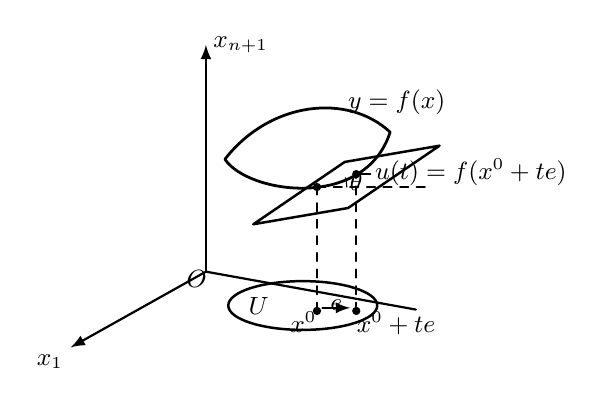
\begin{tikzpicture}[x=0.86cm, y=0.86cm, >=latex, line cap=round, line join=round]
    % ---------- 坐标架 ----------
    \draw[line width=0.8pt, ->] (0, 0) -- (-2.00, -1.12) node[below left=-1pt] {\small $x_{1}$};
    \draw[line width=0.8pt, ->] (0, 0) -- (0, 3.35) node[right=-1pt] {\small $x_{n+1}$};
    \draw[line width=0.8pt] (0, 0) -- (3.10, -0.56);
    \node[below left=-1.5pt, inner sep=1pt] at (0, 0) {\small $O$};
    % ---------- 底面区域 U ----------
    \draw[line width=0.9pt] (1.43, -0.50) ellipse (1.10 and 0.36);
    \node[inner sep=1pt] at (0.78, -0.50) {\small $U$};
    \fill (1.64, -0.58) circle (1.5pt);
    \node[below left=-1.5pt, inner sep=1.5pt] at (1.64, -0.58) {\small $x^{0}$};
    \fill (2.22, -0.58) circle (1.5pt);
    \node[below right=-1.5pt, inner sep=1.5pt] at (2.22, -0.58) {\small $x^{0}+te$};
    \draw[->, line width=0.8pt] (1.72, -0.535) -- (2.13, -0.535);
    \node[above=-2pt, inner sep=1pt] at (1.925, -0.54) {\small $e$};
    % ---------- 竖直虚线与曲面片 ----------
    \draw[line width=0.7pt, dashed] (1.64, -0.58) -- (1.64, 1.25);
    \draw[line width=0.7pt, dashed] (2.22, -0.58) -- (2.22, 1.44);
    % 曲面片 y = f(x)：「透镜」轮廓（下缘经过 A、B）
    \draw[line width=1.0pt]
      (0.28, 1.66)
      .. controls (0.95, 2.52) and (2.10, 2.64) .. (2.72, 2.06)
      .. controls (2.35, 0.90) and (0.62, 1.15) .. (0.28, 1.66);
    \node[anchor=west, inner sep=1pt] at (2.05, 2.50) {\small $y = f(\boldsymbol{x})$};
    % 曲面上的点 A(x^0) 与 B(x^0+te)
    \fill (1.64, 1.25) circle (1.5pt);
    \fill (2.22, 1.44) circle (1.5pt);
    \node[anchor=west, inner sep=1pt] at (2.45, 1.47) {\small $u(t) = f(\boldsymbol{x}^{0} + t\boldsymbol{e})$};
    \draw[line width=0.5pt] (2.43, 1.44) -- (2.24, 1.44);
    % 平面（由 e 方向与竖直方向张成的平行四边形）
    \draw[line width=0.9pt] (0.70, 0.70) -- (2.10, 0.94) -- (3.45, 1.86) -- (2.05, 1.62) -- cycle;
    % 过 A 的水平虚线 与 夹角 theta
    \draw[line width=0.7pt, dashed] (1.64, 1.25) -- (3.25, 1.25);
    \draw (2.08, 1.25) arc[start angle=0, end angle=18.1, radius=0.44];
    \node[inner sep=1pt] at (2.22, 1.33) {\small $\theta$};
  \end{tikzpicture}
  \caption{}\label{fig:8.1.1}
\end{figure}

\begin{example}\label{ex:8.1.1}
设 $\boldsymbol{e}$ 为一个方向, 则 $\|-\boldsymbol{e}\| = \|\boldsymbol{e}\| = 1$, 可见 $-\boldsymbol{e}$ 也为一个方向. 此时, 我们有
\begin{align*}
  \frac{\partial f}{\partial(-\boldsymbol{e})}(\boldsymbol{x}^{0})
  &= \lim_{t \to 0}\frac{f(\boldsymbol{x}^{0} + t(-\boldsymbol{e})) - f(\boldsymbol{x}^{0})}{t}
   = -\lim_{-t \to 0}\frac{f(\boldsymbol{x}^{0} + (-t)\boldsymbol{e}) - f(\boldsymbol{x}^{0})}{-t} \\
  &= -\frac{\partial f}{\partial \boldsymbol{e}}(\boldsymbol{x}^{0}).
\end{align*}
\end{example}

\begin{example}\label{ex:8.1.2}
考察二元函数
\[
  f(x, y) = \begin{cases}
    \dfrac{2xy}{x^{2} + y^{2}}, & (x, y) \neq (0, 0), \\[2.5mm]
    1, & (x, y) = (0, 0).
  \end{cases}
\]
记方向 $\boldsymbol{e} = (\cos\theta, \sin\theta)$, $0 \leqslant \theta < 2\pi$, 并取 $\boldsymbol{x}^{0} = (0, 0)$, 当 $t \neq 0$ 时有
\[
  \frac{f(\boldsymbol{x}^{0} + t\boldsymbol{e}) - f(\boldsymbol{x}^{0})}{t} = \frac{f(t\cos\theta, t\sin\theta) - f(0, 0)}{t} = \frac{2\cos\theta\sin\theta - 1}{t} = \frac{\sin 2\theta - 1}{t}.
\]
由此看出, 当且仅当 $\theta = \dfrac{\pi}{4}$ 与 $\dfrac{5\pi}{4}$, 方向导数存在且为零. 而对其他 $\theta$, 方向导数不存在.
\[
  \begin{aligned}
    \frac{\partial f}{\partial \boldsymbol{e}}(\boldsymbol{x}^{0})
    &= \lim_{t \to 0}\frac{f(\boldsymbol{x}^{0} + t\boldsymbol{e}) - f(\boldsymbol{x}^{0})}{t} = \lim_{t \to 0}\frac{\sin 2\theta - 1}{t} \\
    &= \begin{cases}
         0, & \theta = \dfrac{\pi}{4}\ \text{与}\ \dfrac{5\pi}{4}, \\[3.5mm]
         \infty, & \theta \in \left[0, \dfrac{\pi}{4}\right) \bigcup \left(\dfrac{\pi}{4}, \dfrac{5\pi}{4}\right) \bigcup \left(\dfrac{5\pi}{4}, 2\pi\right).
       \end{cases}
  \end{aligned} \qedhere
\]
\end{example}

记 $\boldsymbol{e}_{i} = (0, 0, \cdots, 0, \underset{\text{第 } i \text{ 个}}{1}, 0, \cdots, 0)$ 为 $\mathbb{R}^{n}$ 中的规范正交基, 即
\[
  \langle \boldsymbol{e}_{i}, \boldsymbol{e}_{j} \rangle = \delta_{ij} = \begin{cases} 1, & i = j, \\ 0, & i \neq j. \end{cases}
\]
设 $\boldsymbol{x}^{0} = (x_{1}^{0}, x_{2}^{0}, \cdots, x_{n}^{0})$, 则
\[
  \begin{aligned}
    \frac{\partial f}{\partial \boldsymbol{e}_{i}}(\boldsymbol{x}^{0})
    &= \lim_{t \to 0}\frac{f(\boldsymbol{x}^{0} + t\boldsymbol{e}_{i}) - f(\boldsymbol{x}^{0})}{t} \\
    &= \lim_{t \to 0}\frac{f(x_{1}^{0}, x_{2}^{0}, \cdots, x_{i-1}^{0}, x_{i}^{0} + t, x_{i+1}^{0}, \cdots, x_{n}^{0}) - f(x_{1}^{0}, x_{2}^{0}, \cdots, x_{n}^{0})}{t} \\
    &= \lim_{x_{i} \to x_{i}^{0}}\frac{f(x_{1}^{0}, x_{2}^{0}, \cdots, x_{i-1}^{0}, x_{i}, x_{i+1}^{0}, \cdots, x_{n}^{0}) - f(x_{1}^{0}, x_{2}^{0}, \cdots, x_{n}^{0})}{x_{i} - x_{i}^{0}} \\
    &\reason{记作} \frac{\partial f}{\partial x_{i}}(\boldsymbol{x}^{0}) = f_{x_{i}}'(\boldsymbol{x}^{0}) = f_{i}'(\boldsymbol{x}^{0}),
  \end{aligned}
\]
称它为 $f$ 的第 $i$ 个\textbf{一阶偏导数}, 它是 $\boldsymbol{x}^{0}$ 点处沿 $\boldsymbol{e}_{i}$ 方向的方向导数.

\begin{example}\label{ex:8.1.3}
在 $\mathbb{R}^{n}$ 中计算函数 $f(\boldsymbol{x}) = \|\boldsymbol{x}\| = \sqrt{x_{1}^{2} + x_{2}^{2} + \cdots + x_{n}^{2}}$ 的偏导数, 其中 $\boldsymbol{x} = (x_{1}, x_{2}, \cdots, x_{n})$.

\begin{solution}
当 $\boldsymbol{x} \neq \boldsymbol{0}$ 时,
\[
  f_{x_{i}}'(\boldsymbol{x}) = \frac{1}{2}(x_{1}^{2} + x_{2}^{2} + \cdots + x_{n}^{2})^{-\frac{1}{2}} \cdot 2x_{i} = \frac{x_{i}}{\|\boldsymbol{x}\|}, \quad i = 1, 2, \cdots, n.
\]
当 $\boldsymbol{x} = \boldsymbol{0}$ 时, 设 $\boldsymbol{e}$ 为任一给定的方向 (单位向量), 此时, 极限
\[
  \lim_{t \to 0}\frac{f(t\boldsymbol{e}) - f(\boldsymbol{0})}{t} = \lim_{t \to 0}\frac{\|t\boldsymbol{e}\|}{t} = \lim_{t \to 0}\frac{|t|\,\|\boldsymbol{e}\|}{t} = \lim_{t \to 0}\frac{|t|}{t}
\]
不存在, 即 $f$ 在原点处的任何方向导数都不存在. 特别地, $f$ 在原点处的任何偏导数也不存在.\qedhere
\end{solution}
\end{example}

如果在开集 $U$ 中的每一点有偏导数, 就得到 $n$ 个一阶偏导函数
\[
  \frac{\partial f}{\partial \boldsymbol{e}_{i}} = \frac{\partial f}{\partial x_{i}}, \quad i = 1, 2, \cdots, n.
\]
如果 $f$ 的一阶偏导函数 $\dfrac{\partial f}{\partial x_{i}}$ 又有偏导数, 称为 $f$ 的\textbf{二阶偏导数}, 记作
\[
  f_{x_{i}x_{j}}'' = \frac{\partial^{2}f}{\partial x_{i}\partial x_{j}} = \frac{\partial}{\partial x_{j}}\Big(\frac{\partial f}{\partial x_{i}}\Big),
\]
\[
  f_{x_{i}x_{i}}'' = \frac{\partial^{2}f}{\partial x_{i}^{2}} = \frac{\partial}{\partial x_{i}}\Big(\frac{\partial f}{\partial x_{i}}\Big), \quad i, j = 1, 2, \cdots, n.
\]
类似可定义 $3$ 阶, $4$ 阶, $\cdots$, $m$ 阶, $\cdots$ 偏导数.

$f$ 为 $C^{k}$ 函数, 即

\noindent $k = 0$, $f$ 连续;

\noindent $0 < k < +\infty$, $f$ 在 $U$ 中有直至 $k$ 阶连续偏导数;

\noindent $k = \infty$, $f$ 在 $U$ 中有各阶连续的偏导数;

\noindent $k = \omega$, $f$ 在 $U$ 中是\textbf{实解析}的, 即 $f$ 在 $U$ 中每一点邻近可展开为收敛的 ($n$ 元) 幂级数:
\[
  f(x_{1}, x_{2}, \cdots, x_{n}) = \sum_{k = 0}^{\infty}\sum_{j_{1}, j_{2}, \cdots, j_{k} = 1}^{n} a_{j_{1}j_{2}\cdots j_{k}}(x_{j_{1}}^{0} - x_{j_{1}})(x_{j_{2}}^{0} - x_{j_{2}})\cdots(x_{j_{k}}^{0} - x_{j_{k}}).
\]
记 $C^{k}(U, \mathbb{R}^{1})$ 为从 $U$ 到 $\mathbb{R}^{1}$ 的 $C^{k}$ 函数的全体.

\begin{theorem}\label{thm:8.1.1}
设 $U \subset \mathbb{R}^{2}$ 为开集, $f: U \to \mathbb{R}^{1}$ 为二元函数. 如果 $f_{xy}''$ 与 $f_{yx}''$ 在 $(x_{0}, y_{0}) \in U$ 连续, 则
\[
  f_{xy}''(x_{0}, y_{0}) = f_{yx}''(x_{0}, y_{0}).
\]
\end{theorem}

\begin{proof}
当 $k \neq 0$, $h \neq 0$ 时, 分别对
\[
  \varphi(y) = f(x_{0} + h, y) - f(x_{0}, y)
\]
与
\[
  \psi(x) = f(x, y_{0} + k) - f(x, y_{0})
\]
应用 Lagrange 中值定理, 就有
\begin{align*}
  &\ [f(x_{0} + h, y_{0} + k) - f(x_{0}, y_{0} + k)] - [f(x_{0} + h, y_{0}) - f(x_{0}, y_{0})] \\
  ={} &\ \varphi(y_{0} + k) - \varphi(y_{0}) = \varphi'(y_{0} + \theta_{1}k)k \\
  ={} &\ [f_{y}'(x_{0} + h, y_{0} + \theta_{1}k) - f_{y}'(x_{0}, y_{0} + \theta_{1}k)]k \\
  ={} &\ f_{yx}''(x_{0} + \theta_{2}h, y_{0} + \theta_{1}k)hk, \quad 0 < \theta_{1}, \theta_{2} < 1.
\end{align*}
另一方面
\begin{align*}
  &\ [f(x_{0} + h, y_{0} + k) - f(x_{0}, y_{0} + k)] - [f(x_{0} + h, y_{0}) - f(x_{0}, y_{0})] \\
  ={} &\ [f(x_{0} + h, y_{0} + k) - f(x_{0} + h, y_{0})] - [f(x_{0}, y_{0} + k) - f(x_{0}, y_{0})] \\
  ={} &\ \psi(x_{0} + h) - \psi(x_{0}) = \psi'(x_{0} + \theta_{3}h)h \\
  ={} &\ [f_{x}'(x_{0} + \theta_{3}h, y_{0} + k) - f_{x}'(x_{0} + \theta_{3}h, y_{0})]h \\
  ={} &\ f_{xy}''(x_{0} + \theta_{3}h, y_{0} + \theta_{4}k)hk, \quad 0 < \theta_{3}, \theta_{4} < 1.
\end{align*}
因此
\[
  f_{xy}''(x_{0} + \theta_{3}h, y_{0} + \theta_{4}k) = f_{yx}''(x_{0} + \theta_{2}h, y_{0} + \theta_{1}k).
\]
由于 $f_{xy}''$ 与 $f_{yx}''$ 在 $(x_{0}, y_{0})$ 处连续, 令 $h \to 0$, $k \to 0$ 就得到
\[
  f_{xy}''(x_{0}, y_{0}) = f_{yx}''(x_{0}, y_{0}). \qedhere
\]
\end{proof}

应用\cref{thm:8.1.1}及归纳法立即可得下面定理.

\begin{theoremp}\label{thm:8.1.1p}
$U \subset \mathbb{R}^{n}$ 为开集, $f: U \to \mathbb{R}^{1}$ 为 $n$ 元函数. 如果 $f$ 在 $U$ 上有直至 $k$ 阶的偏导数, 且都在 $\boldsymbol{x}^{0} = (x_{1}^{0}, x_{2}^{0}, \cdots, x_{n}^{0}) \in U$ 连续, 则
\[
  \frac{\partial^{l}f}{\partial x_{i_{1}}\partial x_{i_{2}}\cdots\partial x_{i_{l}}}(\boldsymbol{x}^{0}) = \frac{\partial^{l}f}{\partial x_{i_{2}}\partial x_{i_{1}}\cdots\partial x_{i_{l}}}(\boldsymbol{x}^{0}) = \cdots = \frac{\partial^{l}f}{\partial x_{i_{l}}\partial x_{i_{l-1}}\cdots\partial x_{i_{1}}}(\boldsymbol{x}^{0}),
\]
即任一 $l\ (\leqslant k)$ 阶偏导数与逐次求导的次序无关.
\end{theoremp}

如果\cref{thm:8.1.1}中条件 ``$f_{xy}''$ 与 $f_{yx}''$ 在 $(x_{0}, y_{0})$ 连续'' 不满足, 则其结论 ``$f_{xy}''(x_{0}, y_{0}) = f_{yx}''(x_{0}, y_{0})$'' 不一定成立.

\begin{example}\label{ex:8.1.4}
设
\[
  f(x, y) = \begin{cases}
    xy\dfrac{x^{2} - y^{2}}{x^{2} + y^{2}}, & (x, y) \neq (0, 0), \\[2.5mm]
    0, & (x, y) = (0, 0),
  \end{cases}
\]
则有
\[
  f_{x}'(0, 0) = \lim_{x \to 0}\frac{f(x, 0) - f(0, 0)}{x - 0} = \lim_{x \to 0}\frac{0 - 0}{x} = \lim_{x \to 0}0 = 0,
\]
\[
  f_{y}'(0, 0) = \lim_{y \to 0}\frac{f(0, y) - f(0, 0)}{y - 0} = \lim_{y \to 0}\frac{0 - 0}{y} = \lim_{y \to 0}0 = 0.
\]
当 $(x, y) \neq (0, 0)$ 时,
\[
  f_{x}'(x, y) = y\left[\frac{x^{2} - y^{2}}{x^{2} + y^{2}} + \frac{4x^{2}y^{2}}{(x^{2} + y^{2})^{2}}\right],
\]
\[
  f_{y}'(x, y) = x\left[\frac{x^{2} - y^{2}}{x^{2} + y^{2}} - \frac{4x^{2}y^{2}}{(x^{2} + y^{2})^{2}}\right].
\]
于是, $\forall y$, $f_{x}'(0, y) = -y$, $f_{xy}''(0, 0) = -1$; $\forall x$, $f_{y}'(x, 0) = x$, $f_{yx}''(0, 0) = 1$,
\[
  f_{xy}''(0, 0) \neq f_{yx}''(0, 0).
\]
由此与\cref{thm:8.1.1}可知, $f_{xy}''$ 与 $f_{yx}''$ 在 $(0, 0)$ 至少有一个不连续.
\end{example}

\begin{example}\label{ex:8.1.5}
设 $f(x, y) = xy$, 求 $f$ 在点 $\boldsymbol{x}^{0} = (1, 1)$ 沿方向 $\boldsymbol{e} = \left(\dfrac{1}{\sqrt{2}}, \dfrac{1}{\sqrt{2}}\right)$ 的方向导数.

\begin{solution}[解法 1]
\[
  \frac{f(\boldsymbol{x}^{0} + t\boldsymbol{e}) - f(\boldsymbol{x}^{0})}{t} = \frac{f\left(1 + \dfrac{t}{\sqrt{2}}, 1 + \dfrac{t}{\sqrt{2}}\right) - f(1, 1)}{t} = \frac{\left(1 + \dfrac{t}{\sqrt{2}}\right)^{2} - 1^{2}}{t} = \sqrt{2} + \frac{t}{2},
\]
\[
  \frac{\partial f}{\partial \boldsymbol{e}}(1, 1) = \lim_{t \to 0}\left(\sqrt{2} + \frac{t}{2}\right) = \sqrt{2}.
\]
\end{solution}

\begin{solution}[解法 2]
\begin{align*}
  \frac{\partial f}{\partial \boldsymbol{e}}(1, 1)
  &= \lim_{t \to 0}\frac{f(\boldsymbol{x}^{0} + t\boldsymbol{e}) - f(\boldsymbol{x}^{0})}{t} \\
  &\reason{\cref{thm:8.1.5}} f_{x}'(1, 1) \cdot \frac{1}{\sqrt{2}} + f_{y}'(1, 1) \cdot \frac{1}{\sqrt{2}} \\
  &= 1 \times \frac{1}{\sqrt{2}} + 1 \times \frac{1}{\sqrt{2}} = \sqrt{2}. \qedhere
\end{align*}
\end{solution}
\end{example}

\begin{example}\label{ex:8.1.6}
设 $f(x, y) = \sqrt{x^{2} + y^{2}} + xy$, 求 $\dfrac{\partial f}{\partial x}(1, 2)$, $\dfrac{\partial f}{\partial y}(1, 2)$.

\begin{solution}
因为
\[
  \frac{\partial f}{\partial x} = \frac{x}{\sqrt{x^{2} + y^{2}}} + y, \qquad \frac{\partial f}{\partial y} = \frac{y}{\sqrt{x^{2} + y^{2}}} + x,
\]
所以
\[
  \frac{\partial f}{\partial x}(1, 2) = \frac{1}{\sqrt{5}} + 2, \qquad \frac{\partial f}{\partial y}(1, 2) = \frac{2}{\sqrt{5}} + 1. \qedhere
\]
\end{solution}
\end{example}

\begin{example}\label{ex:8.1.7}
设 $f(x, y, z) = y^{2}z + \sin 5xy$, 求 $\dfrac{\partial f}{\partial x}$, $\dfrac{\partial f}{\partial y}$, $\dfrac{\partial f}{\partial z}$.

\begin{solution}
$\dfrac{\partial f}{\partial x} = 5y\cos 5xy$, $\dfrac{\partial f}{\partial y} = 2yz + 5x\cos 5xy$, $\dfrac{\partial f}{\partial z} = y^{2}$.\qedhere
\end{solution}
\end{example}

\begin{example}\label{ex:8.1.8}
设 $z = x\ln(1 + x\mathrm{e}^{2y})$, 求 $\dfrac{\partial z}{\partial x}$, $\dfrac{\partial z}{\partial y}$.

\begin{solution}
$\dfrac{\partial z}{\partial x} = \ln(1 + x\mathrm{e}^{2y}) + \dfrac{x\mathrm{e}^{2y}}{1 + x\mathrm{e}^{2y}}$,
\[
  \frac{\partial z}{\partial y} = x \cdot \frac{x\mathrm{e}^{2y} \cdot 2}{1 + x\mathrm{e}^{2y}} = \frac{2x^{2}\mathrm{e}^{2y}}{1 + x\mathrm{e}^{2y}}. \qedhere
\]
\end{solution}
\end{example}

\begin{example}\label{ex:8.1.9}
设 $f(x, y) = xy + 2x^{3}y^{2} + x^{4} + 5$, 求 $f_{xx}''(1, 0)$, $f_{xy}''(1, 0)$, $f_{yx}''(1, 0)$, $f_{yy}''(1, 0)$.

\begin{solution}
$f_{x}'(x, y) = y + 6x^{2}y^{2} + 4x^{3}$, $f_{y}'(x, y) = x + 4x^{3}y$,
\[
  \begin{aligned}
    &f_{xx}''(x, y) = 12xy^{2} + 12x^{2}, \quad f_{xy}''(x, y) = 1 + 12x^{2}y = f_{yx}''(x, y), \\
    &f_{yy}''(x, y) = 4x^{3}.
  \end{aligned}
\]
于是, $f_{xx}''(1, 0) = 12$, $f_{xy}''(1, 0) = 1 = f_{yx}''(1, 0)$, $f_{yy}''(1, 0) = 4$.\qedhere
\end{solution}
\end{example}

回想一元函数 Lagrange 中值定理的推论 3.3.1:

\noindent $f$ 在区间 $I$ 中可导, 则 $f =$ 常数 $\iff f'(x) = 0$, $\forall x \in I$.

能否讲如果 $f'(x) = 0$, 则 $f =$ 常数? 否! 反例:
\[
  f(x) = \begin{cases}
    0, & x \in (-1, 0), \\
    1, & x \in (0, 1).
  \end{cases}
\]
关于 $n$ 元函数, 我们有下面定理.

\begin{theorem}\label{thm:8.1.2}
设 $U \subset \mathbb{R}^{n}$ 为区域, 且对 $\forall \boldsymbol{p} = (x_{1}, x_{2}, \cdots, x_{i-1}, a, x_{i+1}, \cdots, x_{n}) \in U$ 与 $\boldsymbol{q} = (x_{1}, x_{2}, \cdots, x_{i-1}, b, x_{i+1}, \cdots, x_{n}) \in U$, 必有线段 $\overline{\boldsymbol{p}\boldsymbol{q}} = \{(1 - t)\boldsymbol{p} + t\boldsymbol{q} \mid t \in [0, 1]\} \subset U$ (\cref{fig:8.1.2}). 如果 $f$ 在 $U$ 上连续, 且 $\left.\dfrac{\partial f}{\partial x_{i}}\right|_{U} \equiv 0$, 则
\[
  f(x_{1}, x_{2}, \cdots, x_{n}) = \varphi(x_{1}, x_{2}, \cdots, \hat{x}_{i}, \cdots, x_{n}),
\]
即 $f$ 与 $x_{i}$ 无关, 其中 $\hat{x}_{i}$ 表示删去 $x_{i}$.
\end{theorem}

\begin{proof}
固定 $x_{1}, x_{2}, \cdots, x_{i-1}, x_{i+1}, \cdots, x_{n}$, 因为 (不妨设 $a < b$)
\[
  \begin{aligned}
    &\ f(x_{1}, x_{2}, \cdots, x_{i-1}, b, x_{i+1}, \cdots, x_{n}) - f(x_{1}, x_{2}, \cdots, x_{i-1}, a, x_{i+1}, \cdots, x_{n}) \\
    &\reasonb{由 Lagrange 中值定理} {\exists\xi \in (a, b)} \frac{\partial f}{\partial x_{i}}(x_{1}, x_{2}, \cdots, x_{i-1}, \xi, x_{i+1}, \cdots, x_{n})(b - a) \\
    &\ = 0 \cdot (b - a) = 0,
  \end{aligned}
\]
所以, $f(x_{1}, x_{2}, \cdots, x_{n})$ 与 $x_{i}$ 无关.\qedhere
\end{proof}

\textbf{思考题}: 当 $U \subseteq \mathbb{R}^{2}$ 为区域时, 构造反例, 说明\cref{thm:8.1.2}中的结论不成立.

\begin{figure}[htbp]
  \centering
  \begin{tikzpicture}[x=1cm, y=1cm, >=latex, line cap=round, line join=round]
    % 工字形区域
    \fill[pattern=north east lines, pattern color=black!70]
      (-0.72, 1.70) -- (0.72, 1.70) -- (0.72, 1.18) -- (0.36, 1.18) -- (0.36, 0.18)
      -- (1.06, 0.18) -- (1.06, -0.44) -- (-1.06, -0.44) -- (-1.06, 0.18) -- (-0.36, 0.18)
      -- (-0.36, 1.18) -- (-0.72, 1.18) -- cycle;
    \draw[line width=1.0pt]
      (-0.72, 1.70) -- (0.72, 1.70) -- (0.72, 1.18) -- (0.36, 1.18) -- (0.36, 0.18)
      -- (1.06, 0.18) -- (1.06, -0.44) -- (-1.06, -0.44) -- (-1.06, 0.18) -- (-0.36, 0.18)
      -- (-0.36, 1.18) -- (-0.72, 1.18) -- cycle;
    % 上方线段 pq
    \draw[line width=1.4pt] (-0.50, 1.44) -- (0.50, 1.44);
    \fill (-0.50, 1.44) circle (2.0pt);
    \fill (0.50, 1.44) circle (2.0pt);
    \node[above left=-1pt, inner sep=1pt] at (-0.50, 1.46) {\small $p$};
    \node[above right=-1pt, inner sep=1pt] at (0.50, 1.46) {\small $q$};
    % 下方线段
    \draw[line width=1.4pt] (-0.78, -0.13) -- (0.78, -0.13);
    \fill (-0.78, -0.13) circle (2.0pt);
    \fill (0.78, -0.13) circle (2.0pt);
  \end{tikzpicture}
  \caption{}\label{fig:8.1.2}
\end{figure}

\begin{example}\label{ex:8.1.10}
设 $U_{1} = [-2, -1] \times [0, 1]$, $U_{2} = [1, 2] \times [0, 1]$, $U_{3} = [-2, 2] \times [-1, 0]$, $U = U_{1} \cup U_{2} \cup U_{3}$. 显然, $U$ 为 $\mathbb{R}^{2}$ 中的闭区域. 令
\[
  f(x, y) = \begin{cases}
    y^{2}, & (x, y) \in U_{1}, \\
    y^{3}, & (x, y) \in U_{2}, \\
    0, & (x, y) \in U_{3},
  \end{cases}
\]
易见, $f$ 在 $U$ 上连续, $\left.\dfrac{\partial f}{\partial x}\right|_{U} \equiv 0$. 但当 $y = \dfrac{1}{2}$ 时,
\[
  f\Big(x, \frac{1}{2}\Big) = \begin{cases}
    \dfrac{1}{4}, & x \in [-2, -1], \\[2.5mm]
    \dfrac{1}{8}, & x \in [1, 2].
  \end{cases}
\]
这表明函数值与 $x$ 有关 (\cref{fig:8.1.3}).
\end{example}

\begin{figure}[htbp]
  \centering
  \begin{tikzpicture}[x=1cm, y=1cm, >=latex, line cap=round, line join=round]
    % U3 = [-2,2] x [-1,0]：深网点
    \fill[pattern=crosshatch dots, pattern color=black!80, black!25] (-2, -1) rectangle (2, 0);
    \draw[line width=0.8pt] (-2, -1) rectangle (2, 0);
    \node[white, inner sep=1pt] at (-0.78, -0.52) {\small $f = 0$};
    \node[white, inner sep=1pt] at (0.16, -0.52) {\small $U_{3}$};
    % U1 = [-2,-1] x [0,1]
    \fill[pattern=north east lines, pattern color=black!70] (-2, 0) rectangle (-1, 1);
    \draw[line width=0.8pt] (-2, 0) rectangle (-1, 1);
    \node[inner sep=1pt] at (-1.50, 0.26) {\small $U_{1}$};
    % U2 = [1,2] x [0,1]
    \fill[pattern=north east lines, pattern color=black!70] (1, 0) rectangle (2, 1);
    \draw[line width=0.8pt] (1, 0) rectangle (2, 1);
    \node[inner sep=1pt] at (1.50, 0.26) {\small $U_{2}$};
    % y = 1/2 的虚线
    \draw[line width=0.8pt, dashed] (-2, 0.5) -- (-1, 0.5);
    \draw[line width=0.8pt, dashed] (1, 0.5) -- (2, 0.5);
    % 坐标轴
    \draw[line width=0.9pt, ->] (-2.62, 0) -- (2.76, 0) node[below right=-2pt] {\small $x$};
    \draw[line width=0.9pt, ->] (0, -1.30) -- (0, 1.52);
    % 刻度
    \node[left=-2pt, inner sep=1.5pt] at (0, 1) {\small $1$};
    \node[left=-2pt, inner sep=1.5pt] at (0, 0.5) {\small $\frac{1}{2}$};
    \node[below left=-1.5pt, inner sep=1.5pt] at (0, -1) {\small $-1$};
    \node[above left=-1.5pt, inner sep=1.5pt] at (0, 0) {\small $0$};
    \node[below=-2pt, inner sep=1.2pt, fill=white] at (-2, 0) {\small $-2$};
    \node[below=-2pt, inner sep=1.2pt, fill=white] at (-1, 0) {\small $-1$};
    \node[below=-2pt, inner sep=1.2pt, fill=white] at (1, 0) {\small $1$};
    \node[below=-2pt, inner sep=1.2pt, fill=white] at (2, 0) {\small $2$};
    % 标注 f = y^2 / f = y^3
    \node[above=-1pt, inner sep=1pt] at (-1.05, 1.12) {\small $f = y^{2}$};
    \draw[line width=0.6pt] (-1.05, 1.06) -- (-1.30, 0.80);
    \node[above=-1pt, inner sep=1pt] at (1.35, 1.12) {\small $f = y^{3}$};
    \draw[line width=0.6pt] (1.35, 1.06) -- (1.20, 0.80);
    % 标注 f = 1/4 与 f = 1/8
    \node[left=-2pt, inner sep=1pt] at (-2.12, 0.5) {\small $f = \frac{1}{4}$};
    \draw[line width=0.6pt, ->] (-2.06, 0.5) -- (-1.88, 0.5);
    \node[right=-2pt, inner sep=1pt] at (2.12, 0.5) {\small $f = \frac{1}{8}$};
    \draw[line width=0.6pt, ->] (2.06, 0.5) -- (1.88, 0.5);
  \end{tikzpicture}
  \caption{}\label{fig:8.1.3}
\end{figure}

\begin{theorem}\label{thm:8.1.3}
设 $U \subset \mathbb{R}^{n}$ 为开集, $f: U \to \mathbb{R}^{1}$ 为 $n$ 元函数. 如果 $f_{x_{i}}'\ (i = 1, 2, \cdots, n)$ 在 $\boldsymbol{x}^{0} = (x_{1}^{0}, x_{2}^{0}, \cdots, x_{n}^{0}) \in U$ 连续, 则:

(1) $f$ 在 $\boldsymbol{x}^{0}$ 连续;

{\emergencystretch=3em
(2) 如果 $x_{i} = x_{i}(t)\ (i = 1, 2, \cdots, n)$ 在 $t_{0}$ 处可导, 其中 $\boldsymbol{x}^{0} = \boldsymbol{x}(t_{0}) = (x_{1}(t_{0}),\allowbreak x_{2}(t_{0}), \cdots, x_{n}(t_{0}))$, 则对
\[
  \boldsymbol{u} = f(\boldsymbol{x}(t)) = f(x_{1}(t), x_{2}(t), \cdots, x_{n}(t))
\]
有
\[
  \frac{\mathrm{d}u}{\mathrm{d}t}(t_{0}) = \sum_{i = 1}^{n} f_{x_{i}}'\left(\boldsymbol{x}(t_{0})\right)\frac{\mathrm{d}x_{i}}{\mathrm{d}t}(t_{0}).
\]}
\end{theorem}

\begin{proof}
(1) 由 Lagrange 中值定理可知, 存在介于 $x_{i}^{0}$ 与 $x_{i}$ 之间的 $\xi_{i}$, 使得
\begin{align*}
  \lim_{\boldsymbol{x} \to \boldsymbol{x}^{0}} f(\boldsymbol{x})
  &= \lim_{\boldsymbol{x} \to \boldsymbol{x}^{0}}\Biggl\{f(\boldsymbol{x}^{0}) + \sum_{i = 1}^{n}\bigl[f(x_{1}^{0}, x_{2}^{0}, \cdots, x_{i-1}^{0}, x_{i}, \cdots, x_{n}) \\
  &\qquad - f(x_{1}^{0}, x_{2}^{0}, \cdots, x_{i-1}^{0}, x_{i}^{0}, x_{i+1}, \cdots, x_{n})\bigr]\Biggr\} \\
  &= \lim_{\boldsymbol{x} \to \boldsymbol{x}^{0}}\Bigl[f(\boldsymbol{x}^{0}) + \sum_{i = 1}^{n} f_{x_{i}}'(x_{1}^{0}, x_{2}^{0}, \cdots, x_{i-1}^{0}, \xi_{i}, x_{i+1}, \cdots, x_{n})(x_{i} - x_{i}^{0})\Bigr] \\
  &= f(\boldsymbol{x}^{0}) + \sum_{i = 1}^{n} f_{x_{i}}'(\boldsymbol{x}^{0}) \cdot 0 = f(\boldsymbol{x}^{0}),
\end{align*}
即 $f$ 在 $\boldsymbol{x}^{0}$ 处连续.

(2)
\begin{align*}
  \frac{\mathrm{d}u}{\mathrm{d}t}(t_{0})
  &= \lim_{t \to t_{0}}\frac{f(\boldsymbol{x}(t)) - f(\boldsymbol{x}(t_{0}))}{t - t_{0}} \\
  &= \lim_{t \to t_{0}}\sum_{i = 1}^{n} f_{x_{i}}'(x_{1}^{0}, x_{2}^{0}, \cdots, x_{i-1}^{0}, \xi_{i}, x_{i+1}, \cdots, x_{n})\frac{x_{i}(t) - x_{i}(t_{0})}{t - t_{0}} \\
  &= \sum_{i = 1}^{n} f_{x_{i}}'(\boldsymbol{x}(t_{0}))x_{i}'(t_{0}). \qedhere
\end{align*}
\end{proof}

\begin{example}\label{ex:8.1.11}
在\cref{ex:7.5.5}中, 已知
\[
  f(x, y) = \begin{cases}
    \dfrac{xy}{x^{2} + y^{2}}, & (x, y) \neq (0, 0), \\[2.5mm]
    0, & (x, y) = (0, 0)
  \end{cases}
\]
在 $(0, 0)$ 不连续. 由此与\cref{thm:8.1.3}可得 $f_{x}'$ 与 $f_{y}'$ 至少有一个在 $(0, 0)$ 不连续.

另一方面, 从 $f(x, 0) = 0$, $f(0, y) = 0$ 可知, $f_{x}'(0, 0) = 0$, $f_{y}'(0, 0) = 0$. 因此
\[
  f_{x}'(x, y) = \begin{cases}
    \dfrac{y(y^{2} - x^{2})}{(x^{2} + y^{2})^{2}}, & (x, y) \neq (0, 0), \\[2.5mm]
    0, & (x, y) = (0, 0),
  \end{cases}
\]
\[
  f_{y}'(x, y) = \begin{cases}
    \dfrac{x(x^{2} - y^{2})}{(x^{2} + y^{2})^{2}}, & (x, y) \neq (0, 0), \\[2.5mm]
    0, & (x, y) = (0, 0).
  \end{cases}
\]
由于
\[
  \lim_{(x, y) \to (0, 0)} f_{x}'(x, y) = \lim_{(x, y) \to (0, 0)}\frac{y(y^{2} - x^{2})}{(x^{2} + y^{2})^{2}} = \lim_{y \to 0}\frac{1}{y} = \infty \neq 0 = f_{x}'(0, 0),
\]
所以 $f_{x}'$ 在 $(0, 0)$ 点处不连续.

此例表明, 只从 $f_{x}'$ 与 $f_{y}'$ 存在, 而不在 $(0, 0)$ 点连续不能推出 $f$ 在 $(0, 0)$ 点连续. 换句话说, \cref{thm:8.1.3}中条件 ``$f_{x_{i}}'\ (i = 1, 2, \cdots, n)$ 在 $\boldsymbol{x}^{0}$ 连续'' 不能删去.
\end{example}

\begin{theorem}\label{thm:8.1.4}
设 $U \subset \mathbb{R}^{n}$ 为开集, $f: U \to \mathbb{R}^{1}$ 为 $n$ 元函数, $f_{x_{i}}'\ (i = 1, 2, \cdots, n)$ 在 $\boldsymbol{x}^{0} = (x_{1}^{0}, x_{2}^{0}, \cdots, x_{n}^{0})$ 处连续. $x_{i} = x_{i}(\boldsymbol{u}) = x_{i}(u_{1}, u_{2}, \cdots, u_{m})$ 在 $\boldsymbol{u}^{0}$ 有一阶偏导数 $\dfrac{\partial x_{i}}{\partial u_{j}}$, $i = 1, 2, \cdots, n$, $j = 1, 2, \cdots, m$, 且 $\boldsymbol{x}^{0} = \boldsymbol{x}(\boldsymbol{u}^{0})$. 则有多变量的求导链规则:
\[
  \frac{\partial f}{\partial u_{j}}(\boldsymbol{u}^{0}) = \sum_{i = 1}^{n}\frac{\partial f}{\partial x_{i}}(\boldsymbol{x}(\boldsymbol{u}^{0}))\frac{\partial x_{i}}{\partial u_{j}}(\boldsymbol{u}^{0}), \quad j = 1, 2, \cdots, m.
\]
\end{theorem}

\begin{proof}
在\cref{thm:8.1.3}(2) 中, 取 $t = u_{j}$ 即证.\qedhere
\end{proof}

\begin{example}\label{ex:8.1.12}
设一元函数 $f$, $g$ 都二阶可导, 又 $u = u(x, t) = f(x - at) + g(x + at)$, $a$ 为常数. 证明: $u$ 满足二阶偏微分方程
\[
  \frac{\partial^{2}u}{\partial t^{2}} = a^{2}\frac{\partial^{2}u}{\partial x^{2}}.
\]

\begin{proof}
令 $\xi = x - at$, $\eta = x + at$, 则
\[
  \frac{\partial u}{\partial x} = f'(\xi)\frac{\partial\xi}{\partial x} + g'(\eta)\frac{\partial\eta}{\partial x} = f'(x - at) + g'(x + at),
\]
\[
  \frac{\partial u}{\partial t} = f'(\xi)\frac{\partial\xi}{\partial t} + g'(\eta)\frac{\partial\eta}{\partial t} = -af'(x - at) + ag'(x + at),
\]
\[
  \frac{\partial^{2}u}{\partial x^{2}} = f''(x - at) + g''(x + at),
\]
\[
  \frac{\partial^{2}u}{\partial t^{2}} = a^{2}f''(x - at) + a^{2}g''(x + at) = a^{2}\frac{\partial^{2}u}{\partial x^{2}}. \qedhere
\]
\end{proof}
\end{example}

\begin{theorem}\label{thm:8.1.5}
设 $\{\boldsymbol{e}_{i} \mid i = 1, 2, \cdots, n\}$ 为 $\mathbb{R}^{n}$ 中的规范正交基, $\boldsymbol{e} = \sum\limits_{i = 1}^{n}\boldsymbol{e}_{i}\cos\alpha_{i}$ 为单位向量, 此时 $\sum\limits_{i = 1}^{n}\cos^{2}\alpha_{i} = 1$. 如果 $f_{x_{i}}'$ 在 $\boldsymbol{x}^{0}$ 连续, 则 $f$ 在 $\boldsymbol{x}^{0}$ 点沿 $\boldsymbol{e}$ 方向的方向导数为
\[
  \frac{\partial f}{\partial \boldsymbol{e}}(\boldsymbol{x}^{0}) = \sum_{i = 1}^{n}\frac{\partial f}{\partial x_{i}}(\boldsymbol{x}^{0})\cos\alpha_{i}.
\]
这是方向导数用偏导数表达的公式.
\end{theorem}

\begin{proof}
令 $\boldsymbol{x}(t) = \boldsymbol{x}^{0} + t\boldsymbol{e} = \boldsymbol{x}^{0} + t\sum\limits_{i = 1}^{n}\cos\alpha_{i}\boldsymbol{e}_{i}$, $x_{i}(t) = x_{i}^{0} + t\cos\alpha_{i}$, $i = 1, 2, \cdots, n$, 则
\[
  \frac{\partial f}{\partial \boldsymbol{e}}(\boldsymbol{x}^{0}) = \frac{\mathrm{d}}{\mathrm{d}t}f(\boldsymbol{x}^{0} + t\boldsymbol{e})\Big|_{t = 0} \reason{\cref{thm:8.1.4}} \sum_{i = 1}^{n}\frac{\partial f}{\partial x_{i}}(\boldsymbol{x}^{0})\frac{\mathrm{d}x_{i}}{\mathrm{d}t}\Big|_{t = 0} = \sum_{i = 1}^{n}\frac{\partial f}{\partial x_{i}}(\boldsymbol{x}^{0})\cos\alpha_{i}. \qedhere
\]
\end{proof}

在上述定理中, 特别地, 二元函数 $f(x, y)$ 在点 $(x_{0}, y_{0})$ 处沿方向 $\boldsymbol{e} = (\cos\theta, \sin\theta)$ 的方向导数为
\[
  \frac{\partial f}{\partial \boldsymbol{e}}(x_{0}, y_{0}) = \frac{\partial f}{\partial x}(x_{0}, y_{0})\cos\theta + \frac{\partial f}{\partial y}(x_{0}, y_{0})\sin\theta.
\]
三元函数 $f(x, y, z)$ 在点 $(x_{0}, y_{0}, z_{0})$ 处沿方向 $\boldsymbol{e} = (\cos\alpha, \cos\beta, \cos\gamma)$ 的方向导数为
\[
  \frac{\partial f}{\partial \boldsymbol{e}}(x_{0}, y_{0}, z_{0}) = \frac{\partial f}{\partial x}(x_{0}, y_{0}, z_{0})\cos\alpha + \frac{\partial f}{\partial y}(x_{0}, y_{0}, z_{0})\cos\beta + \frac{\partial f}{\partial z}(x_{0}, y_{0}, z_{0})\cos\gamma.
\]

\begin{example}\label{ex:8.1.13}
设 $\boldsymbol{r} = (x, y, z)$, 则 $r = \|\boldsymbol{r}\| = \sqrt{x^{2} + y^{2} + z^{2}}$, 求函数 $r$ 在点 $(x, y, z)$ 沿方向 $\boldsymbol{e} = (\cos\alpha, \cos\beta, \cos\gamma)$ 的方向导数.

\begin{solution}
\begin{align*}
  \frac{\partial r}{\partial \boldsymbol{e}}
  &= \frac{\partial r}{\partial x}\cos\alpha + \frac{\partial r}{\partial y}\cos\beta + \frac{\partial r}{\partial z}\cos\gamma \\
  &= \frac{x}{r}\cos\alpha + \frac{y}{r}\cos\beta + \frac{z}{r}\cos\gamma \\
  &= \frac{\langle \boldsymbol{r}, \boldsymbol{e} \rangle}{\|\boldsymbol{r}\|\,\|\boldsymbol{e}\|} = \cos\theta,
\end{align*}
其中 $\theta$ 为向量 $\boldsymbol{r}$ 与 $\boldsymbol{e}$ 的夹角.\qedhere
\end{solution}
\end{example}

\begin{theorem}\label{thm:8.1.6}
设 $U \subset \mathbb{R}^{n}$ 为开区域, $f$ 在 $\overline{U}$ 上连续, 且于 $U$ 上有 $\dfrac{\partial f}{\partial x_{i}} = 0$, $i = 1, 2, \cdots, n$, 则 $f$ 在 $\overline{U}$ 上为常值函数.
\end{theorem}

\begin{proof}
$\forall \boldsymbol{p} \in U$, 因 $U$ 为开集, 故存在开球 $B(\boldsymbol{p}; \delta) \subset U$. $\forall \boldsymbol{q} \in B(\boldsymbol{p}; \delta)$, 令
\[
  \boldsymbol{u}(t) = f(\boldsymbol{p} + t(\boldsymbol{q} - \boldsymbol{p})) = f((1 - t)\boldsymbol{p} + t\boldsymbol{q}),
\]
则 $u(0) = f(\boldsymbol{p})$, $u(1) = f(\boldsymbol{q})$, $x_{i}(t) = p_{i} + t(q_{i} - p_{i}) = (1 - t)p_{i} + tq_{i}$, $i = 1, 2, \cdots, n$.

由\cref{thm:8.1.3}(2), 有
\begin{align*}
  \frac{\mathrm{d}u}{\mathrm{d}t}
  &= \sum_{i = 1}^{n}\frac{\partial f}{\partial x_{i}}(\boldsymbol{p} + t(\boldsymbol{q} - \boldsymbol{p}))\frac{\mathrm{d}x_{i}}{\mathrm{d}t} \\
  &= \sum_{i = 1}^{n} 0 \cdot (q_{i} - p_{i}) = 0,
\end{align*}
\[
  u(t) = u(0), \quad t \in [0, 1],
\]
\[
  f(\boldsymbol{q}) = u(1) = u(0) = f(\boldsymbol{p}).
\]
所以, $f$ 在 $B(\boldsymbol{p}; \delta)$ 中为常值函数, 从而 $f$ 为局部常值函数.

令
\[
  V = \{\boldsymbol{x} \in U \mid f(\boldsymbol{x}) = f(\boldsymbol{p})\}, \qquad W = \{\boldsymbol{x} \in U \mid f(\boldsymbol{x}) \neq f(\boldsymbol{p})\}.
\]
显然, $\boldsymbol{p} \in V$, 再由 $f$ 为局部常值函数, 故 $V$ 为开集. 从 $f$ 连续推得 $W$ 也为开集. 而 $U = V \cup W$. 由 $U$ 连通立得 $W = \varnothing$, 从而 $U = V$, 即 $f$ 在 $U$ 上为常值函数. 又 $f$ 在 $\overline{U}$ 上连续, 从而 $f$ 在 $\overline{U}$ 上为常值函数.\qedhere
\end{proof}

\begin{remark}\label{rem:8.1.1}
读者可应用 $f$ 局部常值、$U$ 道路连通及有限覆盖定理证明\cref{thm:8.1.6}.
\end{remark}

\begin{definition}\label{def:8.1.2}
设 $U \subset \mathbb{R}^{n}$ 为开集, $f: U \to \mathbb{R}^{1}$ 为 $n$ 元函数. 如果 $\forall t > 0$, $\forall \boldsymbol{x} = (x_{1}, x_{2}, \cdots, x_{n}) \in U$, 必有 $t\boldsymbol{x} \in U$, 且
\[
  f(t\boldsymbol{x}) = f(tx_{1}, tx_{2}, \cdots, tx_{n}) = t^{a}f(\boldsymbol{x}),
\]
则称 $f$ 为 $\alpha$ 次\textbf{齐次函数}.
\end{definition}

\begin{example}\label{ex:8.1.14}
显然, 由\cref{def:8.1.2}可看出
\[
  f(x, y) = 2x^{2} + 6xy - 3y^{2},
\]
$2$ 次齐次函数;
\[
  g(x, y) = \frac{x^{2} + y^{2}}{x + y},
\]
$1$ 次齐次函数;
\[
  h(x, y) = x^{-\frac{1}{2}}\arctan\frac{xy}{x^{2} + y^{2}},
\]
$-\dfrac{1}{2}$ 次齐次函数.
\end{example}

\begin{theorem}[Euler 定理]\label{thm:8.1.7}
设 $U \subset \mathbb{R}^{n}$ 为开集, 且 $\forall t > 0$, $\forall \boldsymbol{x} = (x_{1}, x_{2}, \cdots, x_{n}) \in U$, 必有 $t\boldsymbol{x} \in U$. $f: U \to \mathbb{R}^{1}$ 有连续偏导数 $\dfrac{\partial f}{\partial x_{i}}$, $i = 1, 2, \cdots, n$, 则
\[
  f\ \text{为}\ \alpha\ \text{次齐次函数} \iff \sum_{i = 1}^{n} x_{i}f_{x_{i}}' = \alpha f.
\]
\end{theorem}

\begin{proof}
($\Rightarrow$) 设 $f$ 为 $\alpha$ 次齐次函数, 即 $f(tx_{1}, tx_{2}, \cdots, tx_{n}) = t^{\alpha}f(x_{1}, x_{2}, \cdots, x_{n})$, $\forall t > 0$, $\forall \boldsymbol{x} = (x_{1}, x_{2}, \cdots, x_{n}) \in U$. 上述等式两边对 $t$ 求导得
\[
  \sum_{i = 1}^{n} x_{i}f_{i}'(tx_{1}, tx_{2}, \cdots, tx_{n}) = \alpha t^{\alpha - 1}f(x_{1}, x_{2}, \cdots, x_{n}),
\]
{\emergencystretch=4em
其中 $f_{i}'$ 为 $f$ 关于第 $i$ 个分量的偏导数, 这里不用 $f_{x_{i}}'$ 是防止概念混淆, 如果用 $f_{u_{i}}'(tx_{1}, tx_{2}, \cdots, tx_{n})$, $u_{i} = tx_{i}$ 表示就更确切.\par}

令 $t = 1$ 得到
\[
  \sum_{i = 1}^{n} x_{i}f_{x_{i}}'(x_{1}, x_{2}, \cdots, x_{n}) = \alpha f(x_{1}, x_{2}, \cdots, x_{n}).
\]

($\Leftarrow$) 令
\[
  \varphi(t) = \frac{f(tx_{1}, tx_{2}, \cdots, tx_{n})}{t^{\alpha}}, \quad t > 0,
\]
则
\[
  \begin{aligned}
    \varphi'(t)
    &= \frac{t^{\alpha}\sum\limits_{i = 1}^{n} x_{i}f_{i}'(tx_{1}, tx_{2}, \cdots, tx_{n}) - \alpha t^{\alpha - 1}f(tx_{1}, tx_{2}, \cdots, tx_{n})}{t^{2\alpha}} \\
    &= \frac{\sum\limits_{i = 1}^{n} tx_{i}f_{i}'(tx_{1}, tx_{2}, \cdots, tx_{n}) - \alpha f(tx_{1}, tx_{2}, \cdots, tx_{n})}{t^{\alpha + 1}} = 0,
  \end{aligned}
\]
根据推论 3.3.1, $\varphi(t)$ 当 $t > 0$ 时为常值函数. 所以
\[
  \frac{f(tx_{1}, tx_{2}, \cdots, tx_{n})}{t^{\alpha}} = \varphi(t) = \varphi(1) = f(x_{1}, x_{2}, \cdots, x_{n}),
\]
即
\[
  f(tx_{1}, tx_{2}, \cdots, tx_{n}) = t^{\alpha}f(x_{1}, x_{2}, \cdots, x_{n}), \quad t > 0, \quad \boldsymbol{x} = (x_{1}, x_{2}, \cdots, x_{n}) \in U.
\]
这就证明了 $f$ 为 $\alpha$ 次齐次函数.\qedhere
\end{proof}

\begin{example}\label{ex:8.1.15}
设 $U \subset \mathbb{R}^{3}$ 是关于 $x$, $y$, $z$ 都满足\cref{thm:8.1.2}中条件的区域, $f: U \to \mathbb{R}^{1}$ 有三阶连续的偏导数. 试解方程: $\dfrac{\partial^{3}f}{\partial x\partial y\partial z} = 0$.

\begin{solution}
因为
\[
  0 = \frac{\partial^{3}f}{\partial x\partial y\partial z} = \frac{\partial}{\partial z}\Bigl(\frac{\partial^{2}f}{\partial x\partial y}\Bigr),
\]
故应用\cref{thm:8.1.2}有
\[
  \frac{\partial}{\partial y}\Big(\frac{\partial f}{\partial x}\Big) = \frac{\partial^{2}f}{\partial x\partial y} = \varphi(x, y) \quad (\text{与}\ z\ \text{无关}),
\]
所以
\[
  \frac{\partial f}{\partial x} = \int_{y_{0}}^{y}\varphi(x, y)\,\mathrm{d}y + \psi(x, z),
\]
\[
  f(x, y, z) = \int_{x_{0}}^{x}\left[\int_{y_{0}}^{y}\varphi(x, y)\,\mathrm{d}y\right]\mathrm{d}x + \int_{x_{0}}^{x}\psi(x, z)\,\mathrm{d}x + \theta(y, z).
\]
显然, 当 $\varphi$, $\psi$ 连续时, 上式满足
\[
  \frac{\partial^{3}f}{\partial x\partial y\partial z} = 0. \qedhere
\]
\end{solution}
\end{example}

\begin{exblock}{练习题 8.1}
  \item 计算下列偏导数:

  \begin{tabular}{@{}p{0.44\linewidth}p{0.52\linewidth}@{}}
    (1) $z = e^{xy}$; & (2) $u = \ln(x + y^{2} + z^{3})$; \\
    (3) $z = x^{y}$; & (4) $z = \ln(x_{1} + x_{2} + \cdots + x_{n})$; \\
    (5) $z = \arcsin(x_{1}^{2} + x_{2}^{2} + \cdots + x_{n}^{2})$; & (6) $u = x^{y^{z}}$.
  \end{tabular}

  \item 计算下列偏导数:

  (1) 设 $f(x, y) = x + y + \sqrt{x^{2} + y^{2}}$, 求 $\dfrac{\partial f}{\partial x}(0, 1)$, $\dfrac{\partial f}{\partial y}(0, 1)$;

  (2) 设 $f(x, y) = \ln(1 + xy) + 3$, 求 $\dfrac{\partial f}{\partial x}(1, 2)$, $\dfrac{\partial f}{\partial y}(1, 2)$;

  (3) 设 $f(x, y) = \mathrm{e}^{x + y^{2}} + \sin(x^{2}y)$, 求 $\dfrac{\partial f}{\partial x}(1, 1)$, $\dfrac{\partial f}{\partial y}(1, 1)$.

  \item (1) 设 $f(x, y) = \sqrt{|x^{2} - y^{2}|}$, 问: 在坐标原点处沿哪些方向 $f$ 的方向导数存在?

  (2) 设
  \[
    f(x, y) = \begin{cases}
      \dfrac{xy}{\sqrt{x^{2} + y^{2}}}, & x^{2} + y^{2} \neq 0, \\[2.5mm]
      0, & x^{2} + y^{2} = 0.
    \end{cases}
  \]
  问: 在坐标原点处沿哪些方向 $f$ 的方向导数存在?

  (3) 设 $f(x, y) = \sqrt{x^{2} + y^{2}}$, 试证明 $f(x, y)$ 在点 $(0, 0)$ 连续但偏导数不存在.

  \item 设 $f(x, y) = (x - 1)^{2} - y^{2}$, 求 $f$ 在点 $(0, 1)$ 处沿方向 $\boldsymbol{e} = \left(\dfrac{3}{5}, -\dfrac{4}{5}\right)$ 的方向导数.

  \item 设函数 $f(x, y, z) = |x + y + z|$. 问: 在平面 $x + y + z = 0$ 上的每一点处沿哪些方向 $f$ 存在着方向导数?

  \item 求下列函数的二阶偏导数:

  \begin{tabular}{@{}p{0.44\linewidth}p{0.52\linewidth}@{}}
    (1) $z = xy + \dfrac{x}{y}$; & (2) $z = \tan\dfrac{x^{2}}{y}$; \\[2.5mm]
    (3) $z = \ln(x^{2} + y^{2})$; & (4) $z = \arctan\dfrac{y}{x}$; \\[2.5mm]
    (5) $u = \sin(xyz)$; & (6) $u = xy + yz + zx$; \\
    (7) $u = e^{xyz}$; & (8) $u = x^{yz}$; \\
    (9) $u = \ln(x_{1} + x_{2} + \cdots + x_{n})$; & (10) $u = \arcsin(x_{1}^{2} + x_{2}^{2} + \cdots + x_{n}^{2})$.
  \end{tabular}

  \item 设 $u = \arcsin\dfrac{y}{x}$, 证明: $\dfrac{\partial^{2}u}{\partial x^{2}} + \dfrac{\partial^{2}u}{\partial y^{2}} = 0$.

  \item 设 $u = e^{a\theta}\cos(a\ln r)$, $a$ 为常数. 证明: $\dfrac{\partial^{2}u}{\partial r^{2}} + \dfrac{1}{r^{2}}\dfrac{\partial^{2}u}{\partial \theta^{2}} + \dfrac{1}{r}\dfrac{\partial u}{\partial r} = 0$.

  \item 设 $u = u(x, y, z)$, 令
  \[
    \Delta u = \frac{\partial^{2}u}{\partial x^{2}} + \frac{\partial^{2}u}{\partial y^{2}} + \frac{\partial^{2}u}{\partial z^{2}},
  \]
  我们称
  \[
    \Delta = \frac{\partial^{2}}{\partial x^{2}} + \frac{\partial^{2}}{\partial y^{2}} + \frac{\partial^{2}}{\partial z^{2}}
  \]
  为 \textbf{Laplace 算子}, $\Delta u = 0$ 称为 $u$ 的 \textbf{Laplace 方程}, 满足 Laplace 方程的函数 $u$ 称为\textbf{调和函数}.

  (1) 设 $p = \sqrt{x^{2} + y^{2} + z^{2}}$, 证明:
  \[
    \Delta p = \frac{2}{p}, \quad \Delta\ln p = \frac{1}{p^{2}}, \quad \Delta\Big(\frac{1}{p}\Big) = 0,
  \]
  其中 $p > 0$.

  (2) 设 $u = f(p)$, $f$ 二阶连续可导, 求 $\Delta u$.

  \item 设 $p = \sqrt{x^{2} + y^{2} + z^{2}}$, $u = \dfrac{1}{p}\left[\varphi(p - at) + \psi(p + at)\right]$, $\varphi$ 与 $\psi$ 均二阶连续可导. 证明: $\dfrac{\partial^{2}u}{\partial t^{2}} = a^{2}\Delta u$.

  \item 解下列方程 ($u$ 为 $x$, $y$, $z$ 的函数):

  (1) $\dfrac{\partial^{2}u}{\partial x^{2}} = 0$; \quad (2) $\dfrac{\partial^{2}u}{\partial x\partial y} = 0$; \quad (3) $\dfrac{\partial^{3}u}{\partial x\partial y\partial z} = 0$.

  \item 设二元函数 $f(x, y)$ 在点 $\boldsymbol{x}^{0} = (x_{0}, y_{0})$ 的某开邻域 $U(\boldsymbol{x}^{0})$ 内的偏导函数 $f_{x}'$ 与 $f_{y}'$ 有界, 证明: $f$ 在 $U(\boldsymbol{x}^{0})$ 内连续. 问: 一致连续吗?

  \item 设 $f(x, y, z) = x^{2}y + y^{2}z + z^{2}x$, 证明: $f_{x}' + f_{y}' + f_{z}' = (x + y + z)^{2}$.

  \item 设函数 $u = \ln\dfrac{1}{r}$, $r = \sqrt{(x - a)^{2} + (y - b)^{2} + (z - c)^{2}}$, 求 $u$ 的梯度 $\mathrm{grad}\,u = \left(\dfrac{\partial u}{\partial x}, \dfrac{\partial u}{\partial y}, \dfrac{\partial u}{\partial z}\right)$; 并指出在空间 $\mathbb{R}^{3}$ 的哪些点上成立等式 $|\mathrm{grad}\,u| = 1$.

  \item 设 $u = x^{2} + y^{2} + z^{2} - 3xyz$. 试问: 在怎样的点集上 $\mathrm{grad}\,u$ 分别满足: (1) 垂直于 $x$ 轴; (2) 平行于 $x$ 轴; (3) 恒为零向量.

  \item 设 $r = \sqrt{x^{2} + y^{2} + z^{2}}$, 试求:

  (1) $\mathrm{grad}\,r$; \quad (2) $\mathrm{grad}\,\dfrac{1}{r}$.

  \item 设 $u$, $v$ 为 $x$, $y$, $z$ 的 $C^{1}$ 函数, $f(u)$ 为 $u$ 的 $C^{1}$ 函数, $c$, $\alpha$, $\beta \in \mathbb{R}$ 为常数. 证明:

  (1) $\mathrm{grad}(u + c) = \mathrm{grad}\,u$;

  (2) $\mathrm{grad}(\alpha u + \beta v) = \alpha\,\mathrm{grad}\,u + \beta\,\mathrm{grad}\,v$ (线性性);

  (3) $\mathrm{grad}(uv) = u\,\mathrm{grad}\,v + v\,\mathrm{grad}\,u$ (导性);

  (4) $\mathrm{grad}\,f(u) = f'(u)\,\mathrm{grad}\,u$.

  \item 用多元函数微分法计算下列一元函数的导数:

  (1) $y = x^{x}$; \quad ($y = u^{v}$, $u = x$, $v = x$)

  (2) $y = \dfrac{(1 + x^{2})\ln x}{\sin x + \cos x}$. \quad $\left(y = \dfrac{vw}{u},\ u = \sin x + \cos x,\ v = 1 + x^{2},\ w = \ln x\right)$

  \item 证明: $z = \dfrac{xy^{2}}{\sqrt{x^{2} + y^{2}}} - xy$ 为二次齐次函数.
\end{exblock}

\begin{exblock}{思考题 8.1}
  \item 设 $f(u_{1}, u_{2}, \cdots, u_{n}) = u_{1}u_{2}\cdots u_{n}$, $u_{i} = u_{i}(x)$, 应用多元函数的求导链规则求
  \[
    \frac{\mathrm{d}}{\mathrm{d}x}f(u_{1}(x), u_{2}(x), \cdots, u_{n}(x)).
  \]
  进而证明:
  \[
    \frac{\mathrm{d}}{\mathrm{d}x}
    \left|\begin{matrix}
      a_{11}(x) & \cdots & a_{1n}(x) \\
      \vdots & & \vdots \\
      a_{n1}(x) & \cdots & a_{nn}(x)
    \end{matrix}\right|
    = \sum_{i = 1}^{n}
    \left|\begin{matrix}
      a_{11}(x) & \cdots & a_{1n}(x) \\
      \vdots & & \vdots \\
      a_{i1}'(x) & \cdots & a_{in}'(x) \\
      \vdots & & \vdots \\
      a_{n1}(x) & \cdots & a_{nn}(x)
    \end{matrix}\right|.
  \]

  \item 设
  \[
    \varphi(x, y, z) = \left|\begin{matrix}
      a + x & b + y & c + z \\
      d + z & e + x & f + y \\
      g + y & h + z & i + x
    \end{matrix}\right|,
  \]
  求 $\dfrac{\partial^{2}\varphi}{\partial x^{2}}$.

  \item 设
  \[
    \Phi(x, y, z) = \left|\begin{matrix}
      f_{1}(x) & f_{2}(x) & f_{3}(x) \\
      g_{1}(y) & g_{2}(y) & g_{3}(y) \\
      h_{1}(z) & h_{2}(z) & h_{3}(z)
    \end{matrix}\right|,
  \]
  求 $\dfrac{\partial^{3}\Phi}{\partial x\partial y\partial z}$.

  \item 设
  \[
    u = \left|\begin{matrix}
      1 & 1 & 1 \\
      x & y & z \\
      x^{2} & y^{2} & z^{2}
    \end{matrix}\right|.
  \]
  求: (1) $u_{x}' + u_{y}' + u_{z}'$; \quad (2) $xu_{x}' + yu_{y}' + zu_{z}'$; \quad (3) $u_{xx}'' + u_{yy}'' + u_{zz}''$.

  \item 设 $u = f(x, y)$ 有二阶连续偏导数, $x = r\cos\theta$, $y = r\sin\theta$. 证明:
  \[
    \frac{\partial^{2}u}{\partial r^{2}} + \frac{1}{r}\frac{\partial u}{\partial r} + \frac{1}{r^{2}}\frac{\partial^{2}u}{\partial \theta^{2}} = \frac{\partial^{2}u}{\partial x^{2}} + \frac{\partial^{2}u}{\partial y^{2}}.
  \]

  \item 设 $u = f(r)$ 二阶连续可导, $r^{2} = x_{1}^{2} + x_{2}^{2} + \cdots + x_{n}^{2}$. 证明:
  \[
    \frac{\partial^{2}u}{\partial x_{1}^{2}} + \frac{\partial^{2}u}{\partial x_{2}^{2}} + \cdots + \frac{\partial^{2}u}{\partial x_{n}^{2}} = \frac{\mathrm{d}^{2}u}{\mathrm{d}r^{2}} + \frac{n - 1}{r}\frac{\mathrm{d}u}{\mathrm{d}r}.
  \]

  \item 设 $v = \dfrac{1}{r}g\left(t - \dfrac{r}{c}\right)$, $c \in \mathbb{R}$ 为常数, $r = \sqrt{x^{2} + y^{2} + z^{2}}$, $g$ 为 $C^{2}$ 函数. 证明:
  \[
    v_{xx}'' + v_{yy}'' + v_{zz}'' = \frac{1}{c^{2}}v_{tt}''.
  \]

  \item 证明: 函数
  \[
    u = \frac{1}{2a\sqrt{\pi t}}\mathrm{e}^{-\frac{(x - b)^{2}}{4a^{2}t}} \quad (a, b \in \mathbb{R}\ \text{为常数})
  \]
  满足热传导方程
  \[
    \frac{\partial u}{\partial t} = a^{2}\frac{\partial^{2}u}{\partial x^{2}}.
  \]

  \item 证明: 函数 $u = \ln\sqrt{(x - a)^{2} + (y - b)^{2}}$ ($a$, $b \in \mathbb{R}$ 为常数) 满足 Laplace 方程
  \[
    \Delta u = \frac{\partial^{2}u}{\partial x^{2}} + \frac{\partial^{2}u}{\partial y^{2}} = 0.
  \]

  \item 设函数 $u = f(x, y)$ 为 $C^{2}$ 函数且满足 Laplace 方程
  \[
    \frac{\partial^{2}u}{\partial x^{2}} + \frac{\partial^{2}u}{\partial y^{2}} = 0.
  \]
  证明: 函数 $v = f\left(\dfrac{x}{x^{2} + y^{2}}, \dfrac{y}{x^{2} + y^{2}}\right)$ 也满足 Laplace 方程.

  \item 设 $\varphi$, $\psi$ 为 $C^{2}$ 函数. 证明: 函数 $u = \varphi(x + \psi(y))$ 满足
  \[
    \frac{\partial u}{\partial x}\frac{\partial^{2}u}{\partial x\partial y} = \frac{\partial u}{\partial y}\frac{\partial^{2}u}{\partial x^{2}}.
  \]

  \item 函数的连续性与偏导数存在性两者互不蕴涵.

  (1) 证明:
  \[
    f(x, y) = \begin{cases}
      \mathrm{e}^{-\frac{x^{2}}{y^{2}} - \frac{y^{2}}{x^{2}}}, & xy \neq 0, \\
      0, & xy = 0
    \end{cases}
  \]
  具有各阶偏导数, 但在 $(0, 0)$ 不连续. (这个例子是由 Burr 作出的.)

  (2) 证明:
  \[
    f(x, y) = \begin{cases}
      \mathrm{e}^{x^{-2}y^{-2}/(\mathrm{e}^{x^{-4}} + \mathrm{e}^{y^{-4}})}, & xy \neq 0, \\
      0, & xy = 0
    \end{cases}
  \]
  具有各阶偏导数, 但在 $(0, 0)$ 不连续. (这个例子是由 Snow 作出的.)

  (3) 证明: $f(x, y) = \sqrt{x^{2} + y^{2}}$ 在全平面上连续, 但在 $(0, 0)$ 处两个偏导数不存在.

  \item 研究例子
  \[
    f(x, y) = \begin{cases}
      \dfrac{xy}{x^{2} + y^{2}}, & x^{2} + y^{2} > 0, \\
      0, & x = y = 0
    \end{cases}
  \]
  与
  \[
    f(x, y) = \begin{cases}
      (x + y)\sin\dfrac{1}{x}\sin\dfrac{1}{y}, & x \neq 0,\ y \neq 0,\ x + y \neq 0, \\
      0, & \text{其他},
    \end{cases}
  \]
  说明: 两个累次极限存在且相等与二重极限存在互不蕴涵.
\end{exblock}
